%%%%%%%%%%%%%%%%%%%%%%%%%%%%%%%%%%%%%%%%%%%%%%%%%%%%%%%%%%%%%%%%%%%%%%
% How to use writeLaTeX: 
%
% You edit the source code here on the left, and the preview on the
% right shows you the result within a few seconds.
%
% Bookmark this page and share the URL with your co-authors. They can
% edit at the same time!
%
% You can upload figures, bibliographies, custom classes and
% styles using the files menu.
%
%%%%%%%%%%%%%%%%%%%%%%%%%%%%%%%%%%%%%%%%%%%%%%%%%%%%%%%%%%%%%%%%%%%%%%

\documentclass[12pt]{article}
\usepackage{sbc-template}
\usepackage{graphicx}
\usepackage{url}
\usepackage[brazil]{babel}   
\usepackage[utf8]{inputenc}  
\usepackage{amsmath}
\usepackage{float}
\usepackage{hyperref}
\usepackage{footnote}
\usepackage{threeparttable}


\newtheorem{teorema}{Teorema}
     
\sloppy

\title{Um estudo sobre Lógica Fuzzy e suas Aplicações}

\author{Thiago E. Hamada\inst{1}}

\address{Departamento de Computação -- Universidade Federal de São Carlos
  (UFScar)\\
  Caixa Postal 2645 -- 13560-011 -- São Carlos -- SP -- Brasil
  \email{thiagoeidihamada@gmail.com}
}

\begin{document} 

\maketitle
     
\begin{resumo} 
    Este trabalho apresenta um estudo detalhado sobre a Lógica Fuzzy, abordando seus principais conceitos e definindo como essa teoria se diferencia da lógica tradicional. Inicialmente, são apresentados os fundamentos da Lógica Fuzzy, incluindo conjuntos e regras fuzzy, além das regras de inferência. Em seguida, explora-se suas aplicações no campo da Inteligência Artificial, destacando exemplos práticos e tipos de problemas em que essa lógica se mostra eficaz. Um estudo de caso é apresentado, ilustrando o uso da Lógica Fuzzy no desenvolvimento de sistemas especialistas inteligentes. Na seção de considerações finais, são discutidos os principais pontos positivos e negativos dessa abordagem lógica, comparações com outras lógicas e reflexões pessoais sobre o tema. 
\end{resumo}\newpage

\section{Introdução}
\textit 
O termo fuzzy na língua inglesa pode assumir diferentes significados, dependendo do contexto em que é utilizado, mas seu conceito básico sempre remete à ideia de algo vago, indistinto ou incerto. No português, não há consenso definitivo sobre a melhor tradução, sendo "nebuloso" e "difuso" as opções mais comuns e amplamente aceitas.

A lógica fuzzy, introduzida em 1965 pelo matemático e cientista da computação iraniano Lotfi Zadeh no artigo Fuzzy Sets, surgiu como uma alternativa para superar as limitações da lógica clássica, que trabalha apenas com verdades absolutas (verdadeiro ou falso). Essas limitações ficam evidentes ao tentar modelar situações do mundo real, onde as fronteiras entre categorias nem sempre são nitidamente definidas. Por exemplo, ao considerar a temperatura da água durante um banho, a lógica clássica classificaria a água simplesmente como "fria" ou "quente", sem espaço para variações intermediárias. No entanto, na realidade, a percepção de temperatura é gradual, passando por estágios como "menos fria", "morna" e "quase quente". A lógica fuzzy possibilita justamente esse tipo de raciocínio mais flexível, capaz de lidar com nuances e transições suaves \cite{ZiaeiComparative}

A lógica fuzzy, portanto, representa uma evolução significativa em relação à lógica clássica, proporcionando uma abordagem mais flexível e realista para o raciocínio e a tomada de decisões. Sua capacidade de lidar com incertezas e ambiguidades a torna uma ferramenta poderosa em diversas áreas, como sistemas de controle, inteligência artificial, ciências humanas, medicina, automação industrial, entre outras. Na automação, por exemplo, é amplamente utilizada para otimizar processos, como o controle de temperatura, motores elétricos e sistemas automatizados, garantindo a operação mais eficiente e adaptativa de equipamentos como ar-condicionados, aquecedores e máquinas industriais.

Na indústria automobilística, a lógica fuzzy desempenha um papel crucial em sistemas de controle de tração e estabilidade, na transmissão automática, proporcionando mudanças de marcha suaves e precisas, além de melhorar os sistemas de freios ABS, ajustando automaticamente a pressão dos freios para aumentar a segurança. No setor agrícola, sua aplicação em sistemas de irrigação inteligente ajuda a otimizar o uso da água com base na umidade do solo e nas condições climáticas, e também auxilia na modelagem ambiental, ajudando a prever fenômenos naturais e mitigar riscos.

No setor da saúde, a lógica fuzzy é empregada em sistemas de apoio ao diagnóstico médico, oferecendo uma análise mais precisa, mesmo quando os sintomas são imprecisos ou subjetivos. Também é utilizada no controle de equipamentos médicos, como bombas de infusão e ventiladores mecânicos, garantindo maior segurança e conforto para os pacientes. Nas telecomunicações, contribui para o gerenciamento inteligente de redes, otimizando o tráfego de dados e aprimorando algoritmos de compressão de áudio e vídeo, o que melhora a qualidade e a eficiência das transmissões. Em eletrodomésticos inteligentes, como máquinas de lavar e fornos micro-ondas, a lógica fuzzy permite ajustes automáticos no tempo de operação, consumo de água e controle de temperatura, proporcionando maior conveniência e economia de recursos.

No campo das finanças e economia, a lógica fuzzy é utilizada para a análise de riscos e na modelagem preditiva de mercados, permitindo avaliações mais robustas em cenários com alta variabilidade e incerteza. No transporte e na logística, sua aplicação inclui sistemas de semáforos inteligentes, que ajustam automaticamente os tempos de sinal com base no fluxo de tráfego, e algoritmos de roteirização, que otimizam as rotas levando em consideração fatores como trânsito, condições climáticas e distância.

Ao romper com os sistemas binários tradicionais, a lógica fuzzy abriu novas possibilidades na era digital, consolidando-se como um pilar da tecnologia moderna e ampliando os horizontes para soluções inovadoras e adaptativas em um mundo cada vez mais complexo e dinâmico. Neste artigo, exploraremos a evolução da lógica fuzzy, suas principais aplicações e sua influência em diversas áreas do conhecimento, destacando sua importância como uma extensão da lógica clássica e sua relevância para o futuro da tecnologia e da ciência.

Neste artigo, o estudo será focado nos fundamentos e nas aplicações da lógica fuzzy no âmbito da inteligência artificial, explorando como essa abordagem pode aprimorar sistemas inteligentes, permitir a tomada de decisões em cenários complexos e contribuir para o desenvolvimento de algoritmos mais adaptativos e eficientes. Serão abordados desde os conceitos teóricos até exemplos práticos, destacando o papel da lógica fuzzy em áreas como aprendizado de máquina, sistemas especialistas, reconhecimento de padrões e robótica, evidenciando seu potencial transformador na criação de soluções tecnológicas avançadas.

\section{Fundamentos da Lógica Fuzzy}

\subsection{Comparação Lógica Convencional x Lógica Fuzzy}

Como mostrado anteriormente, ao contrário da Lógica convencional, a Lógica Fuzzy parte da ideia de que características como temperatura, altura, velocidade, entre outras, podem ter graus de pertinência. Dessa forma, a Lógica Fuzzy busca modelar o sentido das palavras, a tomada de decisões e o raciocínio comum do ser humano. De forma ilustrativa, considere o gráfico mostrado Figura \ref{fig:fig1}, que representa um exemplo típico da teoria clássica e descreve a altura de uma pessoa por meio de três conjuntos: baixo, médio e alto. Nesse exemplo, dado um valor qualquer para x, ele pertencente a um dos conjuntos do gráfico; por exemplo, se x = 1,65, então x pertence ao conjunto médio e não aos outros. Ou seja, um elemento pertence ou não a um determinado conjunto, e, além disso, não pode pertencer a mais de um conjunto simultaneamente.

\begin{figure}[ht]
\centering
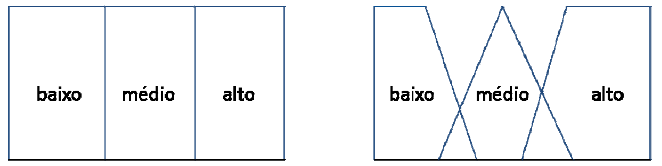
\includegraphics[width=.9\textwidth]{CompareClassicFuzzy.png}
\caption{Representação na forma de conjuntos da altura de uma pessoa, sob o
ponto de vista da Lógica convencional (à esquerda) e do da Lógica Fuzzy (à direita)}
{\footnotesize Fonte \cite{ConceitFuzzy}}
\label{fig:fig1}
\end{figure}

Um outro exemplo que destaca as limitações da lógica clássica é a velocidade em uma rodovia. Na lógica tradicional, poderíamos definir que dirigir abaixo de 100 km/h é "lento" e acima de 100 km/h é "rápido". No entanto, essa abordagem é simplista, pois ignora a gradualidade entre os extremos. Na lógica fuzzy, podemos definir que abaixo de 70 km/h a velocidade é "lenta", acima de 130 km/h é "rápida", e entre 70 e 130 km/h a velocidade é uma combinação de "lenta" e "rápida", refletindo melhor a maneira como o cérebro humano processa informações 

Esses exemplos ilustram dois conceitos-chave da lógica fuzzy:

    Pertinência a múltiplos conjuntos: Diferente da lógica clássica, onde um valor pertence exclusivamente a um conjunto, na lógica fuzzy um valor pode pertencer a vários conjuntos simultaneamente. Por exemplo, 90 km/h pode ser considerado parcialmente "lento" e parcialmente "rápido", dependendo do contexto.

    Regras de inferência fuzzy: A lógica fuzzy utiliza regras do tipo "Se..., então..." para modelar decisões. Por exemplo, no caso da gorjeta em um restaurante, poderíamos ter uma regra como: "Se o serviço foi muito bom E a comida foi média E eu estou de bom humor, então a gorjeta será alta". Essas regras permitem combinar múltiplas variáveis, como qualidade do serviço, qualidade da comida e humor, para tomar decisões mais complexas e realistas.

Além disso, a lógica fuzzy utiliza funções lógicas como "E" (interseção) e "OU" (união) para combinar critérios. Por exemplo, no caso da gorjeta, a função "E" exige que todos os critérios sejam atendidos simultaneamente, enquanto a função "OU" permite que pelo menos um dos critérios seja satisfeito. Essas funções são fundamentais para modelar decisões multifatoriais, que são comuns em situações reais.

Esses aspecto são importantes pela necessidade de atribuir valores ou pontuações às variáveis envolvidas nas regras. No caso da altura de uma pessoa ou da velocidade na rodovia, isso é relativamente simples, pois ambas podem ser medidas em escalas numéricas (Metros ou km/h). No entanto, em situações como a avaliação da qualidade do serviço em um restaurante, é necessário criar escalas subjetivas (por exemplo, de 0 a 10) e interpretar esses valores de forma consistente.

\subsection{Fuzzyficação}

"A fuzzyficação é o processo de converter um valor numérico de entrada em graus de pertinência a diferentes conjuntos fuzzy".\cite{youtubeFuzzy} Esses conjuntos representam categorias linguísticas, como "Baixo", "Médio" ou "Alto", e são definidos por funções de pertinência que determinam o grau em que um valor pertence a cada conjunto. O grau de pertinência varia no intervalo [0,1]: um valor de 0 significa que o elemento não pertence ao conjunto fuzzy, um valor de 1 indica pertencimento total, e qualquer valor entre 0 e 1 representa um grau intermediário de associação, refletindo a incerteza ou gradualidade da classificação. 

\newpage

\begin{figure}[ht]
\centering
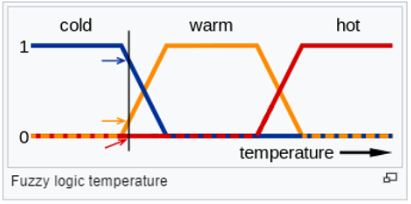
\includegraphics[width=.7\textwidth]{FuzzyficaçãoTemp.png}
\caption{Representação de conjuntos fuzzy para a temperatura}
{\footnotesize Fonte \cite{ZiaeiComparative}}
\label{fig:fig2}
\end{figure}

Por exemplo, na Figura 2, onde os termos linguísticos "Frio", "Morno" e "Quente" são representados por funções de pertinência. Cada função mapeia o grau de pertencimento de uma temperatura específica a cada um desses conjuntos fuzzy. Suponha que uma linha vertical na escala marque uma temperatura de 15°C, e que três setas indiquem os graus de pertinência correspondentes:

    A seta azul aponta para 0,8 na função "Frio", indicando que essa temperatura tem uma pertinência alta no conjunto fuzzy "Frio", ou seja, é "bastante fria".
    A seta laranja aponta para 0,2 na função "Morno", sugerindo que essa temperatura é apenas "levemente morna".
    A seta vermelha aponta para 0, o que significa que a temperatura não pertence ao conjunto fuzzy "Quente", sendo "nada quente".

Esses graus de pertinência (0,8 para "Frio", 0,2 para "Morno" e 0 para "Quente") são o resultado direto do processo de fuzzyficação, convertendo o valor nítido da temperatura em uma representação difusa que permite raciocinar de forma mais flexível e próxima ao pensamento humano.

\subsection{Conjuntos Fuzzy e Graus de Pertinência}

"Um conjunto fuzzy é uma classe de objetos com um contínuo de graus de pertencimento. Tal conjunto é caracterizado por uma função de pertencimento (ou característica) que atribui a cada objeto um grau de pertencimento variando entre zero e um. As noções de inclusão, união, interseção, complemento, relação, convexidade, etc., são estendidas a tais conjuntos, e várias propriedades dessas noções no contexto dos conjuntos fuzzy são estabelecidas. Em particular, um teorema de separação para conjuntos fuzzy convexos é provado sem exigir que os conjuntos fuzzy sejam disjuntos."\cite{ZADEH1965338}

Dessa forma um conjunto Fuzzy é definido como um par $(U, m)$, onde $U$ é o universo de discurso (um conjunto de referência) e $m$ é a função de pertinência. A função de pertinência $m_A$ atribui a cada elemento $x$ em $U$ um grau de pertencimento ao conjunto fuzzy $A = (U, m)$, que pode variar de 0 (não pertencente) a 1 (pertencimento total), ou qualquer valor intermediário (pertencimento parcial).

\begin{figure}[ht]
\centering
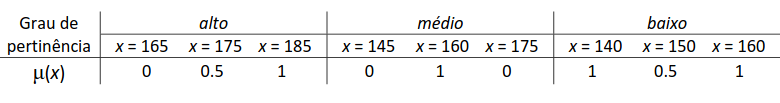
\includegraphics[width=.9\textwidth]{ConjFuzzy.png}
\caption{Altura: conjuntos fuzzy e graus de pertinência para alguns valores de x}
{\footnotesize Fonte \cite{ConceitFuzzy}}
\label{fig:fig3}
\end{figure}

Para um conjunto finito $U = \{x_1, \dots, x_n\}$, o conjunto fuzzy $(U, m)$ pode ser representado como $\{m(x_1)/x_1, \dots, m(x_n)/x_n\}$. Dependendo do valor de $m(x)$, um elemento $x$ pode ser classificado como:

\begin{itemize}
  \item Não incluído: $m(x) = 0$
  \item Totalmente incluído: $m(x) = 1$
  \item Parcialmente incluído: $0 < m(x) < 1$
\end{itemize}

Os conjuntos crisp associados a um conjunto fuzzy $A = (U, m)$ incluem:

\begin{itemize}
  \item Corte alfa: $\alpha A = \{x \in U \mid m(x) \geq \alpha\}$
  \item Corte alfa forte: $A'_{\alpha} = \{x \in U \mid m(x) > \alpha\}$
  \item Suporte: $\text{Supp}(A) = \{x \in U \mid m(x) > 0\}$
  \item Núcleo: $\text{Core}(A) = \{x \in U \mid m(x) = 1\}$

A altura de um conjunto fuzzy A é o maior valor da função de pertinência, denotado por Hgt(A) = sup{mA(x) | x em U}. Um conjunto fuzzy é considerado normalizado se sua altura for igual a 1.
\end{itemize}

\subsection{Operadores Fuzzy}

Os operadores fuzzy são conceitos cruciais na teoria dos conjuntos fuzzy, que surgiu como uma extensão da lógica tradicional para lidar com a incerteza e a imprecisão inerentes ao mundo real. Em contraste com a lógica clássica, que opera com valores binários (0 ou 1), a lógica fuzzy permite que os valores de pertinência variem contínuamente entre 0 e 1, o que possibilita representar a gradatividade de pertencimento de um elemento a um conjunto. Esses operadores são fundamentais para modelar e processar informações que não podem ser descritas de maneira exata ou precisa, como conceitos vagos, subjetivos ou imprecisos.

\begin{figure}[ht]
\centering
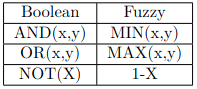
\includegraphics[width=.4\textwidth]{OperadoresFuzzy.png}
\caption{Comparação de Operadores Booleanos e Fuzzy}
{\footnotesize Fonte \cite{ZiaeiComparative}
\label{fig:fig4}
\end{figure}

Os principais operadores fuzzy incluem a união (ou "ou fuzzy"), que combina dois conjuntos fuzzy e atribui a cada elemento o maior grau de pertinência entre os dois conjuntos. Isso reflete a ideia de que, para que um elemento pertença a um conjunto, basta que ele pertença, de forma significativa, a um dos conjuntos envolvidos. A interseção (ou "e fuzzy") determina o grau de pertinência de um elemento ao selecionar o menor grau de pertinência entre os conjuntos envolvidos, refletindo a ideia de que um elemento precisa atender simultaneamente aos critérios de ambos os conjuntos para ser considerado pertencente a ambos. A complementação (ou "não fuzzy") inverte o grau de pertinência de um elemento, representando a ideia de negação fuzzy. Isso significa que, se um elemento tem um grau de pertinência de 0,7 em um conjunto fuzzy, seu grau de pertinência no conjunto complementar será 0,3, ao invés de ser simplesmente 1, como acontece na lógica booleana.

Além desses operadores básicos, também existem operadores de implicação e agregação que são utilizados para lidar com relações mais complexas entre conjuntos fuzzy e são especialmente úteis em sistemas de inferência fuzzy. A implicação fuzzy é utilizada para representar relações de causa e efeito, enquanto a agregação permite combinar múltiplos graus de pertinência provenientes de diferentes fontes ou critérios.

Esses operadores são fundamentais em uma vasta gama de aplicações, especialmente em sistemas de controle fuzzy, onde são usados para modelar e controlar processos com base em informações imprecisas, como a temperatura em um forno ou a velocidade de um veículo. São também essenciais em áreas como inteligência artificial, onde ajudam na tomada de decisões em cenários de incerteza, e em sistemas de recomendação, diagnóstico médico, processamento de linguagem natural, entre outros. A capacidade dos operadores fuzzy de lidar com incertezas e complexidades permite que sistemas computacionais sejam desenvolvidos para imitar a forma como seres humanos pensam e tomam decisões em situações imprecisas, tornando-os extremamente poderosos para resolver problemas que envolvem variabilidade e subjetividade.

\subsection{Inferência Fuzzy}

Após a fuzzificação, os valores fuzzy passam pelo processo de inferência, onde um conjunto de regras fuzzy define a relação entre as variáveis de entrada e a saída do sistema. Essas regras são expressas no formato:

    SE (Condição 1) E/OU (Condição 2), ENTÃO (Saída esperada).

Considere um sistema de controle de velocidade de um ventilador baseado na temperatura ambiente:

    Regra 1: Se a temperatura for "Frio", então a velocidade do ventilador será "Baixa".
    
    Regra 2: Se a temperatura for "Morno", então a velocidade será "Média".
    
    Regra 3: Se a temperatura for "Quente", então a velocidade será "Alta".

A aplicação dessas regras é realizada por meio dos operadores fuzzy, previamente discutidos. Cada regra gera um grau de ativação com base nos valores fuzzy da entrada e nos operadores aplicados, resultando em um conjunto fuzzy para a saída. Esse conjunto pode incluir múltiplos graus de pertinência em diferentes categorias de saída, exigindo um processo de agregação para consolidar a resposta do sistema.

O resultado dessa etapa ainda se mantém no domínio fuzzy, exigindo a aplicação de um método de desfuzzificação para converter os valores difusos em um valor numérico exato, adequado para controle e tomada de decisão prática.

\subsection{Desfuzzificação}

A desfuzzificação é o processo de transformar os resultados fuzzy, que são expressos em termos de graus de pertinência, em valores concretos e definitivos, que podem ser utilizados em um sistema de decisão ou controle. Em outras palavras, após as regras fuzzy serem aplicadas e gerar valores como "um pouco alto" ou "médio", a desfuzzificação converte esses valores em números que podem ser facilmente compreendidos e utilizados.

Existem vários métodos para fazer a desfuzzificação, mas o mais comum é o método do centro de gravidade. Nesse método, imaginamos que os diferentes valores fuzzy representam uma distribuição de peso, como se fossem partes de uma forma. O centro de gravidade dessa forma nos dá o valor final, que é o valor numérico correspondente ao resultado fuzzy.

Por exemplo, se a combinação das regras fuzzy deu como resultado um "médio" em uma variável, que tem um grau de pertinência de 0.7, e um "alto" em outra variável, com um grau de 0.5, a desfuzzificação calcula um valor numérico que leva em consideração esses graus de pertinência para chegar a um número único, como 6 ou 7. Esse número é o valor final do sistema, que pode ser usado em decisões práticas, como ajustar a temperatura de um forno ou a velocidade de um motor.

De forma simples, a desfuzzificação pega a "fuzzy" resposta do sistema e a transforma em um valor claro e útil para a aplicação real.

\section{Aplicações em Inteligência Artificial}

A lógica fuzzy é essencial para a inteligência artificial porque permite que sistemas computacionais lidem com incerteza, imprecisão e subjetividade de forma mais próxima à maneira como os humanos tomam decisões. Como dito anteriormente, a lógica clássica, opera apenas com valores binários (0 ou 1, verdadeiro ou falso), diferente da lógica fuzzy que trabalha com graus de verdade, possibilitando respostas mais flexíveis e adaptáveis. \cite{inbook}

Algumas das principais aplicações incluem:

Sistemas Especialistas e Diagnóstico Médico
    A lógica fuzzy permite a criação de sistemas especialistas que auxiliam na tomada de decisão em ambientes onde as regras não são exatas.
    No setor da saúde, a lógica fuzzy é usada para diagnosticar doenças com base em sintomas subjetivos, como dor, fadiga e desconforto, ajudando médicos a tomar decisões mais informadas.

Controle de Sistemas Autônomos e Robótica
    Veículos autônomos utilizam lógica fuzzy para interpretar cenários de trânsito e tomar decisões em tempo real, como ajuste de velocidade e frenagem em situações de risco.
    Robôs industriais e assistentes domésticos empregam lógica fuzzy para ajustar seus movimentos de forma precisa, mesmo diante de variações inesperadas no ambiente.

Sistemas de Recomendação Fuzzy
    Plataformas de streaming e e-commerce utilizam lógica fuzzy para analisar preferências dos usuários de maneira mais flexível, oferecendo recomendações personalizadas mesmo quando há poucas informações disponíveis.

Processamento de Linguagem Natural (PLN)
    A lógica fuzzy melhora o entendimento da linguagem humana em assistentes virtuais e chatbots, permitindo uma interpretação mais próxima da linguagem natural, levando em conta ambiguidades e contextos diferentes.

Aprendizado de Máquina Fuzzy
    No aprendizado de máquina, modelos baseados em lógica fuzzy ajudam a interpretar e classificar dados ruidosos de forma mais eficiente. Técnicas como redes neurais fuzzy combinam a capacidade de aprendizado das redes neurais com a interpretabilidade dos sistemas fuzzy.
    
Segurança Cibernética e Detecção de Anomalias
    A lógica fuzzy é usada em sistemas de segurança para identificar ataques cibernéticos, analisando padrões anômalos de tráfego de rede e classificando ameaças com base em um grau de certeza.

\subsection{Framework do Aprendizado de Máquina Fuzzy}
A lógica fuzzy tem sido amplamente integrada a técnicas de aprendizado de máquina, formando o campo do Fuzzy Machine Learning (FML). A figura 5 estrutura o aprendizado de máquina fuzzy em cinco principais categorias:

\begin{figure}[ht]
\centering
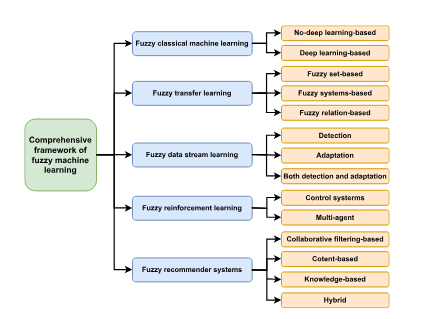
\includegraphics[width=.8\textwidth]{FrameworkFuzzy.png}
\caption{Framework do Aprendizado de Máquina Fuzzy}
{\footnotesize Fonte \cite{10496855}
\label{fig:fig4}
\end{figure}

\subsubsectionFuzzy{Fuzzy Classical Machine Learning}

Modelos tradicionais de aprendizado de máquina podem ser aprimorados com lógica fuzzy para lidar com incerteza e imprecisão nos dados. Esses modelos podem ser categorizados em abordagens que utilizam ou não aprendizado profundo. A lógica fuzzy melhora a interpretabilidade dos modelos ao permitir que as decisões sejam tomadas com base em graus de verdade, em vez de valores estritamente binários. Isso torna esses métodos particularmente úteis em aplicações onde os dados possuem incerteza ou ambiguidade, como em diagnósticos médicos e previsão de séries temporais.

\subsubsectionFuzzy{Transfer Learning}

O aprendizado por transferência fuzzy aplica técnicas que permitem reutilizar conhecimento previamente adquirido em um domínio para melhorar o aprendizado em outro. Esse método é especialmente útil quando há escassez de dados no novo domínio, permitindo que um modelo pré-treinado seja adaptado de maneira eficiente. A lógica fuzzy é utilizada para lidar com variações entre os domínios, reduzindo a discrepância entre os conjuntos de dados e permitindo uma adaptação mais flexível. Aplicações incluem reconhecimento de padrões, tradução automática e adaptação de modelos para diferentes populações em sistemas biomédicos.

\subsubsection{Fuzzy Data Stream Learning}

Esse método se refere ao aprendizado contínuo a partir de fluxos de dados dinâmicos, onde os padrões podem mudar ao longo do tempo. A lógica fuzzy auxilia na detecção e adaptação a essas mudanças, permitindo que os modelos se ajustem automaticamente a novos padrões sem a necessidade de recomeçar o treinamento do zero. Essa abordagem é crucial para sistemas que operam em tempo real, como análise de dados de sensores, monitoramento de fraudes financeiras e sistemas de previsão climática.

\subsubsection{Fuzzy Reinforcement Learning}

O aprendizado por reforço fuzzy combina técnicas de aprendizado baseado em recompensas com lógica fuzzy para tomada de decisões mais flexíveis e interpretáveis. Esse método é amplamente utilizado em controle de sistemas autônomos, como veículos autônomos e robótica, onde as ações precisam ser ajustadas continuamente com base em um ambiente dinâmico e incerto. Além disso, é aplicado em ambientes multiagentes, onde diferentes agentes inteligentes precisam interagir e cooperar, como em jogos estratégicos, automação industrial e sistemas de negociação financeira.

\subsubsection{Fuzzy Recommender Systems}

Os sistemas de recomendação fuzzy utilizam lógica fuzzy para lidar com a subjetividade e a incerteza na modelagem das preferências dos usuários. Esses sistemas combinam abordagens híbridas, como filtragem colaborativa, análise baseada em conteúdo e sistemas baseados em conhecimento. A lógica fuzzy permite capturar nuances nas preferências dos usuários e oferecer recomendações mais precisas e personalizadas. Aplicações incluem plataformas de streaming, e-commerce, sistemas educacionais personalizados e recomendação de tratamentos médicos.

\section{Considerações Finais}

A lógica fuzzy tem se consolidado como uma ferramenta essencial para a Inteligência Artificial, principalmente em aplicações que envolvem incerteza e tomada de decisão em ambientes dinâmicos. Sua capacidade de lidar com graus de verdade permite a criação de sistemas mais flexíveis e interpretáveis, ampliando suas aplicações em diversas áreas, como controle de sistemas autônomos, aprendizado de máquina, processamento de linguagem natural e sistemas de recomendação.

\subsection{Pontos Positivos}
\subsubsection{Complementaridade e Flexibilidade da Lógica Fuzzy}
A lógica fuzzy expande os métodos clássicos ao proporcionar maior flexibilidade no tratamento de informações imprecisas e incertas.\cite{book} Diferente das abordagens binárias ou logísticas estritas, ela permite modelagens mais próximas da complexidade do mundo real, capturando nuances e ambiguidades que seriam perdidas em sistemas rígidos. Essa característica torna a lógica fuzzy uma alternativa poderosa para lidar com cenários onde a incerteza e a subjetividade desempenham um papel central.
\subsubsection{Diversidade de Aplicações Práticas}
A versatilidade da lógica fuzzy se reflete em uma ampla gama de aplicações, demonstrando sua eficácia em diferentes áreas. Desde sistemas de controle avançados até a interpretação de comportamentos e decisões humanas não determinísticas, essa abordagem se mostra essencial para modelar fenômenos complexos. Seu uso abrange setores como inteligência artificial, automação industrial, diagnóstico médico, entre outros, evidenciando sua adaptabilidade a contextos diversos.

\subsection{Pontos Negativos}

\subsubsection{Escalabilidade limitada}
Em sistemas de grande escala, a lógica fuzzy pode não escalar bem. Quando muitas variáveis e regras são introduzidas, a complexidade aumenta exponencialmente. Isso pode tornar o sistema lento ou difícil de gerenciar.

\subsubsection{Dificuldade de modelagem}
Definir as funções de pertinência e as regras fuzzy de forma eficaz pode ser desafiador. A escolha inadequada desses elementos pode levar a um desempenho insatisfatório do sistema, e o processo de otimização dessas variáveis pode exigir muita experimentação e conhecimento do domínio.

\subsection{Discussão}

A lógica fuzzy, apesar de ser um modelo bastante útil para representar incertezas e informações imprecisas, levanta várias questões interessantes em relação à sua aplicação e comparação com outras abordagens. Aqui estão algumas discussões que podem proporcionar uma compreensão mais profunda do tema:

\subsubsection{Pertinência vs. Probabilidade}

Uma das questões centrais ao se estudar a lógica fuzzy é a comparação entre pertinência e probabilidade. Ambos lidam com a incerteza, mas de formas diferentes:

Pertinência na lógica fuzzy é um valor que indica o grau com que um elemento pertence a um conjunto fuzzy. Esse grau é um número entre 0 e 1, onde 0 significa "nenhuma pertinência" e 1 significa "total pertinência". Por exemplo, no conjunto "alto", uma pessoa com 1,80m pode ter uma pertinência de 0,8, o que indica que ela não é totalmente "alta", mas se aproxima disso.

Probabilidade, por outro lado, é usada para modelar a chance de um evento ocorrer. Ela também é representada por um número entre 0 e 1, mas está relacionada a um fenômeno de incerteza que pode ser repetido. Probabilidades são associadas à ocorrência de eventos específicos e são baseadas em modelos estatísticos de incerteza.

Podemos concluir, portanto, que pertinência lida com a associação de um elemento a um conjunto fuzzy em um único contexto, a probabilidade está associada à chance de ocorrência de um evento e é baseada em dados e fenômenos estocásticos. A lógica fuzzy não garante um comportamento repetitivo, como a probabilidade. Isso significa que, em um sistema fuzzy, a pertinência de um valor não reflete necessariamente uma repetição ou uma chance futura, mas sim uma descrição de seu grau de adequação a um conceito vago.

\subsection{Pontos de Interesse}
A aplicação da lógica fuzzy na inteligência artificial se destaca por sua capacidade de lidar com a incerteza e a subjetividade, algo que os sistemas tradicionais de lógica binária não conseguem fazer com tanta eficiência. O mais interessante é como essa abordagem permite que máquinas tomem decisões de maneira mais próxima ao raciocínio humano, utilizando graus de verdade em vez de apenas "verdadeiro" ou "falso". Isso é especialmente útil em áreas como sistemas especialistas, controle de processos industriais, reconhecimento de padrões e até em veículos autônomos.

Outro ponto fascinante é a flexibilidade que a lógica fuzzy oferece para modelar problemas complexos sem exigir um conhecimento exato das variáveis envolvidas. Diferente de métodos puramente estatísticos ou baseados em aprendizado profundo, a lógica fuzzy pode ser interpretada e ajustada com regras compreensíveis, tornando-a uma ferramenta poderosa para especialistas em diversas áreas.

\subsection{Dificuldades encontradas}

A necessidade de interpretar e validar os resultados, diferente de abordagens mais matemáticas, onde os cálculos seguem uma estrutura bem definida, a lógica fuzzy pode gerar saídas que precisam de uma análise subjetiva, o que pode dificultar a automação completa de algumas tarefas.

Além disso, muitos artigos acadêmicos relevantes estão restritos a plataformas pagas, limitando o acesso a quem não possui assinaturas institucionais ou individuais. Isso torna a busca por referências confiáveis mais trabalhosa, exigindo a exploração de repositórios gratuitos, não muito pertinentes com a pesquisa.


\bibliographystyle{sbc}
\bibliography{sbc-template}

\end{document}
